\documentclass[10pt]{article}

% --- Packages ---
\usepackage[utf8]{inputenc}
\usepackage[T1]{fontenc}
\usepackage[margin=1.55cm,top=1.15cm,bottom=1.35cm]{geometry}
\usepackage{times}
\usepackage{amsmath,amssymb}
\usepackage{booktabs}
\usepackage{tabularx}
\usepackage{array}
\usepackage{graphicx}
\usepackage{tikz}
\usetikzlibrary{arrows.meta,positioning,fit,backgrounds,shapes.geometric}
\usepackage{algorithm}
\usepackage{algpseudocode}
\usepackage{enumitem}
\usepackage{hyperref}
\usepackage{caption}
\usepackage{titlesec}
\usepackage{xcolor}
\usepackage{float}
\usepackage{balance}

% --- Compact formatting for the six double-column pages ---
\setlength{\parskip}{1pt plus 0.5pt}
\setlength{\parindent}{0pt}
\setlength{\columnsep}{0.55cm}
\setlength{\abovedisplayskip}{2pt}
\setlength{\belowdisplayskip}{2pt}
\setlength{\intextsep}{3pt plus 1pt minus 1pt}
\setlength{\floatsep}{3pt plus 1pt minus 1pt}
\setlength{\textfloatsep}{3pt plus 1pt minus 1pt}
\titlespacing*{\section}{0pt}{5pt}{2pt}
\titlespacing*{\subsection}{0pt}{3pt}{1pt}
\titleformat{\section}{\normalfont\bfseries\normalsize}{\thesection.}{0.4em}{}
\titleformat{\subsection}{\normalfont\bfseries\small}{\thesubsection.}{0.3em}{}
\setlist{nosep,leftmargin=*,topsep=0pt,parsep=0pt}
\captionsetup{font=small,labelfont=bf,skip=2pt}
\makeatletter
\renewcommand{\ALG@beginalgorithmic}{\scriptsize}
\def\input@path{{./}{report/}}
\makeatother

% --- White placeholders: figures/graphs will be inserted later ---
\newcommand{\whiteplaceholder}[2]{%
  \begin{center}
  \fcolorbox{black}{white}{\rule{0pt}{#2}\rule{#1}{0pt}}
  \end{center}%
}
\newcolumntype{Y}{>{\raggedright\arraybackslash}X}

\begin{document}

% ---------------------------------------------------------------------------
% Cover page. The six-page limit applies after this cover.
% ---------------------------------------------------------------------------
\begin{titlepage}
\thispagestyle{empty}
\centering
\vspace*{1.6cm}
{\LARGE\bfseries Nature@Cloud\\[3pt]Final Project Report\par}
\vspace{0.6cm}
{\large Cloud Computing and Virtualization, 2025--26, IST\par}
\vspace{0.35cm}
{\normalsize Group 35\par}
\vspace{0.35cm}
{\normalsize
Lu\'is Rosa (ist1116307)\quad
Laura Rodrigues (ist1116260)\quad
Jo\~ao Guerreiro (ist1116375)\par}
\vfill
\begin{minipage}{0.86\textwidth}
\textbf{Abstract.}
Nature@Cloud is an elastic AWS service for three parameterized, compute-intensive workloads inspired by natural systems: Julia-set fractals, Gray--Scott reaction-diffusion, and DNA matching. The central problem is to minimize request latency and cloud cost while requests have highly variable complexity and while wall-clock time becomes unreliable under concurrent execution. Our solution uses a custom Java Load Balancer and Auto-Scaler running on EC2, instrumented EC2 workers, optional Lambda workers for short overflow/fallback requests, and DynamoDB as a Metrics Storage System. The Load Balancer estimates each request's work before dispatch using historical Javassist metrics and calibrated parameter heuristics; the Auto-Scaler converts that estimated work into seconds on \texttt{t3.micro} workers and scales EC2 capacity with hysteresis.
\end{minipage}
\vfill
\textbf{Video:} \url{https://youtu.be/PLACEHOLDER}
\end{titlepage}

\clearpage
\setcounter{page}{1}
\twocolumn

\section{Problem Framing and Solution}

Nature@Cloud receives HTTP requests for three workloads whose parameters change the amount of CPU work and memory pressure by several orders of magnitude. A small DNA request can finish in milliseconds, while a Gray--Scott simulation may execute tens of billions of bytecode instructions. Static request counts are therefore a poor scheduling signal: one request may be cheap, while another can saturate a \texttt{t3.micro} worker for tens of seconds. Raw processing time is also unsuitable as a primary metric because it depends on contention, JIT warm-up, burst credits, and co-located requests.

The project requirement is an elastic cloud architecture with EC2 workers, Lambda workers, a custom Load Balancer (LB), a custom Auto-Scaler (AS), and a DynamoDB Metrics Storage System (MSS). Our design uses \emph{estimated work} as the common abstraction across all components. EC2 workers run the Nature@Cloud web server with a Javassist Java agent; each completed request writes metrics to DynamoDB. The LB estimates the next request from its type and parameters, chooses EC2 or Lambda, and tracks the work currently assigned to each VM. The AS reads the same in-flight work counters and starts or terminates EC2 workers to balance latency and cost.

\begin{figure}[H]
\centering
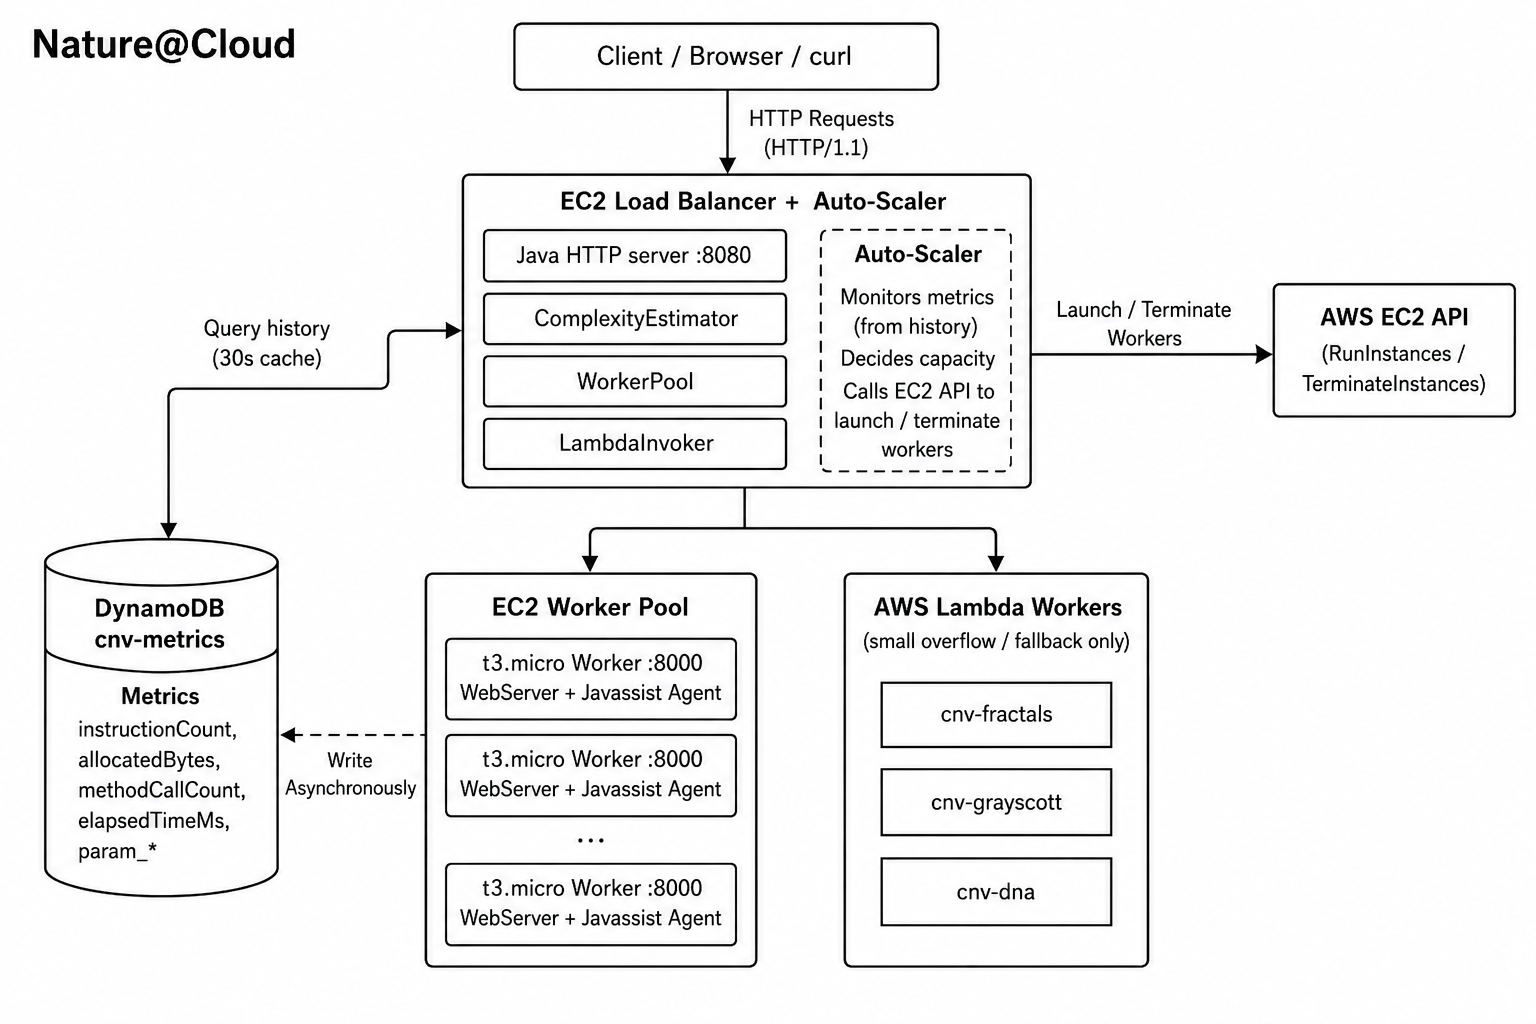
\includegraphics[width=\linewidth]{figures/architecture.png}
\caption{Nature@Cloud system architecture.}
\label{fig:architecture}
\end{figure}

\begin{table}[H]
\centering
\scriptsize
\caption{Workloads and request parameters used as LB input.}
\begin{tabularx}{\columnwidth}{@{}lYY@{}}
\toprule
Type & Main parameters & Output \\
\midrule
\texttt{fractals} & \texttt{w}, \texttt{h}, \texttt{iterations} & PNG encoded as data URI \\
\texttt{grayscott} & \texttt{size}, \texttt{maxIterations}, \texttt{f}, \texttt{k}, \texttt{stopOnExtinction}, \texttt{seedMode} & PNG encoded as data URI \\
\texttt{dna} & \texttt{seq1}, \texttt{seq2}, \texttt{minLength}, \texttt{stopOnFirst} & HTML match report \\
\bottomrule
\end{tabularx}
\end{table}

\section{Distributed Architecture}

\textbf{Workers.} VM workers are \texttt{t3.micro} EC2 instances running a Java \texttt{HttpServer} on port \texttt{8000} with a cached thread pool. They expose \texttt{/fractals}, \texttt{/grayscott}, \texttt{/dna}, and \texttt{/} for health checks. The worker AMI contains Java, the application JARs, and a \texttt{systemd} service so new instances boot directly into the instrumented server. Lambda workers are deployed as three Java 11 functions, \texttt{cnv-fractals}, \texttt{cnv-grayscott}, and \texttt{cnv-dna}, with 512 MB and a 120 s function timeout; the LB uses a stricter 5 s eligibility threshold, so large requests are never sent to Lambda.

\textbf{Load Balancer and Auto-Scaler.} The LB is a Java web server on a dedicated EC2 instance, listening on port \texttt{8080}; it is the only client-facing entry point. The AS is co-located with the LB, which the assignment allows, and uses the AWS EC2 SDK to discover, launch, and terminate workers. Both components share the \texttt{WorkerPool}, where each worker record stores endpoint, instance id, active-request count, and accumulated estimated work of currently assigned requests.

\textbf{MSS and deployment.} DynamoDB table \texttt{cnv-metrics} stores one item per completed EC2 request. Deployment is automated through ordered, idempotent scripts for IAM, network/security groups, AMI creation, initial worker, LB, Lambdas, and cleanup. The cleanup script is part of the operational design because the project uses real AWS resources and VPCs, EC2 instances, AMIs, and DynamoDB tables should not remain allocated after sessions.

\section{Instrumentation, Metrics, and MSS}

\subsection{Javassist Instrumentation}

The Java agent instruments only workload packages (fractals, Gray--Scott, and DNA), excluding the JDK, AWS SDK, HTTP framework, and image libraries. This keeps the signal focused on workload complexity and avoids paying overhead for code that the scheduler should not model.

The primary CPU metric is dynamic bytecode instruction count, \texttt{instruction\allowbreak Count}. For each method, the agent uses Javassist \texttt{ControlFlow.basicBlocks()} to find real basic blocks, counts the number $N$ of original bytecode instructions in each block, and injects:
\[
\texttt{MetricRegistry.incrementInstructions(}N\texttt{)}.
\]
The call executes every time the block is visited, so loops are counted dynamically. This gives more precision than counting every block as one unit while avoiding one instrumentation call per bytecode instruction. A method-entry counter, \texttt{method\allowbreak Call\allowbreak Count}, is kept only as a diagnostic cross-check.

Per-request isolation is implemented with \texttt{ThreadLocal\allowbreak\textless Request\allowbreak Metrics\textgreater}. Handler methods are wrapped with \texttt{startRequest(uri)} and \texttt{stopRequest()}, resetting counters at the beginning of each request and snapshotting them at completion. This prevents metrics from concurrent requests or previous requests from mixing.

\subsection{Composite Work Metric}

Scheduling uses a composite cost:
\[
\hat{C} = W_{CPU}\cdot \widehat{ICount} + W_{RAM}\cdot \widehat{AllocBytes},
\]
with default $W_{CPU}=W_{RAM}=1.0$, configurable through \texttt{-Dcnv.\allowbreak estwork.\allowbreak wcpu} and \texttt{-Dcnv.\allowbreak estwork.\allowbreak wram}. \texttt{AllocatedBytes} is collected per thread using \texttt{ThreadMXBean.getThreadAllocatedBytes()}, so no extra bytecode instrumentation is needed for memory.

ICount is the dominant signal for fractals and Gray--Scott, which are CPU-bound. RAM is still useful because it captures an independent dimension: fractal memory scales mainly with $w\cdot h$, Gray--Scott memory with $size^2$, and DNA can allocate many bytes despite few instructions. Thus the composite metric is CPU-driven for current workloads but extensible to memory-heavy requests.

\begin{figure}[H]
\whiteplaceholder{0.88\columnwidth}{0.66\columnwidth}
\caption{Placeholder for metric-justification graphs: (a) workload feature vs. measured ICount, (b) ICount/composite cost vs. wall-clock on \texttt{t3.micro}, and (c) instrumentation overhead comparing no agent, method-only, basic-block count, and basic-block ICount.}
\label{fig:metrics}
\end{figure}

\subsection{DynamoDB Schema and Cache}

The MSS stores what is needed to estimate future requests, not just logs. Each item has partition key \texttt{requestType}, sort key \texttt{requestId} (timestamp plus short UUID), numeric metrics \texttt{instruction\allowbreak Count}, \texttt{allocatedBytes}, \texttt{method\allowbreak Call\allowbreak Count}, \texttt{elapsedTimeMs}, \texttt{timestamp}, and all original query parameters under \texttt{param\_*}. Workers enqueue metric writes in memory and flush them every 15 s with DynamoDB \texttt{BatchWriteItem} batches of up to 25 items. This keeps user responses off the DynamoDB critical path and reduces per-request SDK/HTTP overhead while preserving one historical record per request. The table uses PAY\_PER\_REQUEST billing and workers degrade to local-only metrics if DynamoDB is unavailable.

The LB does not query DynamoDB exhaustively for every request. \texttt{ComplexityEstimator} keeps a local read-through cache keyed by \texttt{requestType}. Each cache entry stores up to the 50 most recent historical records for that workload and has a 30 s TTL; empty histories are also cached, and DynamoDB reconnect is retried at most once per 60 s while unavailable. This avoids making the MSS a bottleneck.

The cache is not an exact-parameter memoization table. A new request with, for example, size 10001 can benefit from records with size 10000 because the estimator converts parameters into continuous workload features and learns ratios between feature values and measured work. Similar parameters therefore produce similar estimates even when the exact tuple has never appeared.

\section{Complexity Estimation}

For request parameters $p=(t,\theta)$, where $t$ is the workload type and $\theta$ is the map of query parameters, the estimator first tries a history-based model. For each historical record $i$ of type $t$, it computes a feature $f_i=f(t,\theta_i)$ and ratios $r^C_i=ICount_i/f_i$, $r^R_i=AllocBytes_i/f_i$. For the new request:
\[
\widehat{ICount}=\overline{r^C}\,f(t,\theta),\quad
\widehat{AllocBytes}=\overline{r^R}\,f(t,\theta).
\]
If no valid history exists, or DynamoDB is unavailable, calibrated heuristics are used.

\begin{table}[H]
\centering
\scriptsize
\caption{Estimator features and cold-start heuristics.}
\begin{tabularx}{\columnwidth}{@{}lYY@{}}
\toprule
Type & CPU feature / heuristic & RAM heuristic \\
\midrule
Fractals & $w\cdot h\cdot \min(iter,500)$; multiplier 10, 5, or 2 for low/mid/high iteration regimes & $33\cdot w\cdot h$ bytes \\
Gray--Scott & $size^2\cdot maxIter\cdot 164$ & $64\cdot size^2$ bytes \\
DNA & $17\cdot seedScan + 60\cdot(|seq1|+|seq2|)$ & $52\cdot seedScan + 480\cdot(|seq1|+|seq2|)$ bytes \\
\bottomrule
\end{tabularx}
\end{table}

The features are based on empirical calibration. Gray--Scott is the strongest case: $size^2\cdot maxIter$ yields about 164 instructions per cell-iteration from $64^2\times1000$ to $384^2\times2000$. Fractals scale linearly with $w\cdot h$ for fixed iteration count, but Julia-set bailout saturates empirically near 500 iterations for the provided constant, so the feature caps \texttt{iterations}. DNA is the exception to the one-feature model: two requests with the same lengths may differ by over $100\times$ depending on whether seeds from \texttt{seq1} occur in \texttt{seq2}. We therefore use a lightweight \emph{seedScan} feature: build a set of \texttt{minLength}-seeds from \texttt{seq2}; for each seed of \texttt{seq1}, add 1 if present and add a full-scan cost otherwise. This approximates failed \texttt{findSeed} scans without executing the full matcher, and the sequence-length term covers parsing, matched arrays, and HTML output.

\section{Load Balancing and Lambda Policy}

The LB receives \texttt{type\_parameters} $p=(t,\theta)$ for every request. $W$ is the set of currently healthy EC2 worker records in the \texttt{WorkerPool}; each $w\in W$ has load $L(w)$, the sum of estimated costs of in-flight requests assigned to it. $E$ is the set of workers already tried for this request.

\begin{algorithm}[H]
\caption{Cost-aware routing with EC2 retry and Lambda fallback}
\label{alg:lb}
\begin{algorithmic}[1]
\Procedure{Route}{$p=(t,\theta)$, $W$}
  \State $\hat{C} \gets \Call{EstimateCost}{t,\theta}$
  \State $s \gets \hat{C}/(2.0\times10^6\cdot1000)$ \Comment{estimated seconds}
  \If{$s\leq5$ \textbf{and} all $w\in W$ have $L(w)>0.8\cdot MAXCAP$}
    \State try Lambda$(t,\theta)$; if it succeeds, return response
  \EndIf
  \State $E\gets\emptyset$
  \For{$attempt=1$ to $\min(3,|W|)$}
    \State $w\gets\Call{SelectWorker}{W\setminus E,\hat{C}}$
    \If{$w=\bot$}
      \State \textbf{break}
    \EndIf
    \State $E\gets E\cup\{w\}$; $L(w)\gets L(w)+\hat{C}$
    \State forward request to $w$ with 120 s timeout
    \State $L(w)\gets L(w)-\hat{C}$
    \If{transport succeeded}
      \State return worker response
    \EndIf
  \EndFor
  \If{$s\leq5$}
    \State try Lambda$(t,\theta)$ as last resort
  \EndIf
  \State return \texttt{502} if all eligible paths failed
\EndProcedure
\Procedure{SelectWorker}{$Cands,\hat{C}$}
  \State choose the most-loaded $w$ with $L(w)+\hat{C}\leq MAXCAP$
  \If{no such worker exists}
    \State choose the least-loaded $w\in Cands$
  \EndIf
  \State \Return chosen worker or $\bot$
\EndProcedure
\end{algorithmic}
\end{algorithm}

The worker selection intentionally combines packing and spreading. Pure spreading reduces short-term latency but keeps every VM slightly busy, which delays scale-down and increases EC2 cost. Pure packing minimizes cost but may overload one worker. Our policy packs while the projected work remains under $MAXCAP=5\times10^{10}$ composite units (25 s on calibrated \texttt{t3.micro}), then falls back to least-loaded spreading so the request is still served and the AS observes overload.

Lambda is a pressure valve, not the primary path. EC2 is preferred for sustained work because a warm VM is cheaper per continuous workload. Lambda is used only for requests estimated at at most 5 s when every EC2 worker is above 80\% of the per-worker cap, or after EC2 retries fail. This avoids launching a 30--60 s EC2 cold start for a small burst, while ensuring very large requests never go to Lambda.

\section{Auto-Scaling and Fault Tolerance}

The AS runs every 5 s and maintains 1--5 workers. It computes the average percentage of calibrated worker capacity currently occupied by in-flight work:
\[
avgCapacity(\%)=100\cdot\frac{\sum_{w\in W}L(w)}{|W|\cdot MAXCAP}.
\]
Here $MAXCAP=5\times10^{10}$ composite units corresponds to 25 s of work on the calibrated \texttt{t3.micro}. Scale-up occurs above 80\% average capacity; scale-down occurs below 20\%, with a 60 s cooldown. The 80\% threshold leaves roughly 20\% headroom before the per-worker packing cap, while the 20\% scale-down threshold requires the cluster to become substantially idle before terminating VMs. This 4$\times$ hysteresis avoids oscillation.

\begin{table}[H]
\centering
\scriptsize
\caption{Auto-scaler constants and rationale.}
\begin{tabularx}{\columnwidth}{@{}lYY@{}}
\toprule
Parameter & Value & Rationale \\
\midrule
Per-worker cap & 100\% $=5\times10^{10}$ & 25 s of calibrated \texttt{t3.micro} work \\
Scale-up & 80\% avg. capacity & Equivalent to 20 s/worker \\
Scale-down & 20\% avg. capacity & Equivalent to 5 s/worker \\
Packing cap & 100\% per worker & About one heavy Gray--Scott request \\
Cooldown & 60 s & Avoid EC2 churn \\
Drain & 15 polls $\times$ 2 s & Avoid voluntary termination during active work \\
\bottomrule
\end{tabularx}
\end{table}

\begin{algorithm}[H]
\caption{Auto-scaling over worker set $W$}
\label{alg:as}
\begin{algorithmic}[1]
\Procedure{CheckAndScale}{$W$}
  \State $A\gets\Call{AvgCapacityPercent}{W}$
  \If{cooldown active}
    \State \Return
  \EndIf
  \If{$|W|<1$}
    \State launch EC2 worker
  \ElsIf{$A>80\%$ \textbf{and} $|W|<5$}
    \State launch EC2 worker
  \ElsIf{$A<20\%$ \textbf{and} $|W|>1$}
    \State $w\gets$ least-loaded AutoScaler-managed worker
    \State remove $w$ from LB pool so it receives no new requests
    \For{$i=1$ to $15$}
      \If{$active(w)=0$}
        \State terminate EC2 instance
        \State \Return
      \EndIf
      \State sleep 2 s
    \EndFor
    \State re-add $w$; defer termination to a later cycle
  \EndIf
\EndProcedure
\end{algorithmic}
\end{algorithm}

Fault tolerance is layered. At request level, transport exceptions or timeouts cause the LB to retry on different EC2 workers, excluding already-tried workers. If all EC2 attempts fail, Lambda is tried only when the request is Lambda-eligible; otherwise the LB returns an error rather than executing a large request in Lambda. At VM level, health checks run every 15 s and remove a worker after three consecutive failed probes to \texttt{/}. The AS callback then terminates the corresponding EC2 instance so failed workers do not become orphaned paid resources. If the pool drops below the minimum, the AS launches a replacement worker. Voluntary scale-down is drain-first: a worker is removed from selection, observed for active requests, and only terminated when no active request is recorded.

\begin{figure}[H]
\whiteplaceholder{0.88\columnwidth}{0.58\columnwidth}
\caption{Placeholder for autoscaling and fault-tolerance graphs: worker count over time during a burst, average capacity utilization (\%), scale-up/scale-down percentage thresholds, retries, and health-check evictions.}
\label{fig:autoscale}
\end{figure}

\section{Evaluation and Design Justification}

\textbf{Metric correlation.} Local calibration used 33 image/simulation requests plus a focused DNA feature benchmark with 24 requests. Gray--Scott showed an almost constant ratio of about 164 instructions per cell-iteration: $64^2\times1000$ produced 673.6M instructions, $128^2\times2000$ produced 5.38B, and $384^2\times2000$ produced 48.39B. Fractals showed that $w\cdot h$ is linear at fixed iteration count, while \texttt{iterations} saturates: for $w=h=400$, 500, 1000, and 2000 iterations all measured 140.7M instructions. DNA required two signals: simple length/product features had low explanatory power ($R^2\approx0.22$--$0.29$), while \emph{seedScan} reached $R^2=0.999$ for \texttt{instructionCount}; adding sequence size captures memory/output behavior.

\textbf{Memory contribution.} RAM calibration supports separate CPU and RAM reasoning. Fractals allocate about 33 B/pixel and Gray--Scott about 64 B/cell. For DNA, allocation is driven both by failed seed scans, which create substring/compare work, and by sequence/output size; the focused benchmark showed \emph{seedScan} also correlating with \texttt{allocatedBytes} ($R^2=0.992$). For current CPU-bound workloads, ICount dominates the composite value (e.g., Gray--Scott $256^2\times5000$ has 53.77B instructions versus about 4.05 MB allocated), but DNA demonstrates that memory pressure can be a meaningful second signal.

\textbf{Threshold calibration.} The AS thresholds are expressed as percentages of calibrated per-worker capacity. Eight representative AWS requests gave mean throughput near $2.0\times10^6$ instr/ms, so $MAXCAP=5\times10^{10}$ represents about 25 s on a \texttt{t3.micro}. We set scale-up to 80\% of this cap, i.e., about 20 s of pending work per worker, and scale-down to 20\%, i.e., about 5 s. These percentages are interpretable, independent of the raw metric scale, and tied to workload behavior: the 100\% cap matches one heavy Gray--Scott request, the 80\% trigger leaves headroom for arrivals, and the 20\% lower threshold avoids flapping.

\begin{table}[H]
\centering
\scriptsize
\caption{Representative evidence used to configure the system.}
\begin{tabularx}{\columnwidth}{@{}lYY@{}}
\toprule
Question & Evidence & Decision \\
\midrule
Does ICount predict work? & Gray--Scott ratio $\approx164$ across $10^9$--$10^{10}$ instructions & Use $size^2\cdot maxIter$ and ICount as primary CPU metric \\
Do fractal iterations scale forever? & $400^2$ at 500, 1000, 2000 iterations all $140.7$M instr. & Cap feature at 500 iterations \\
Why two DNA signals? & Same-size DNA requests differed by $>100\times$; \emph{seedScan} gave $R^2=0.999$ & Use seed-search + memory/output features \\
When scale? & 25 s calibrated cap per worker & Use 80\% / 20\% utilization thresholds \\
\bottomrule
\end{tabularx}
\end{table}

\begin{figure}[H]
\whiteplaceholder{0.88\columnwidth}{0.60\columnwidth}
\caption{Placeholder for final experimental graphs: ICount-feature regression per workload, RAM-feature regression, LB routing decisions under mixed workloads, and EC2-vs-Lambda cost/latency comparison.}
\label{fig:eval}
\end{figure}

\textbf{AWS validation.} The deployment pipeline was validated end-to-end in \texttt{eu-west-1}. The documented run created IAM/network resources, built an AMI, launched one LB and one worker, and served all three workload endpoints through the LB with HTTP 200. DynamoDB stored request metrics with the final \texttt{instruction\allowbreak Count} schema, the estimator later used history mode, AutoScaler scale-up was observed under parallel Gray--Scott load, and scale-down returned the pool to one worker after load stopped. Lambda integration is implemented and deployed by \texttt{06-deploy-\allowbreak lambdas.\allowbreak sh}; routing uses the policy in Algorithm~\ref{alg:lb}.

\textbf{Limitations.} The LB is a single point of failure, as allowed by the assignment. The estimator currently uses the same feature for CPU and RAM history ratios, although RAM sometimes scales with a simpler feature; because RAM is small for the dominant workloads, this has limited impact, and separate RAM features are future work. \texttt{t3.micro} instances are burstable, so sustained baseline throughput can fall below the calibrated burst throughput; the AS mitigates this by scaling before one worker accumulates long queues. Worker transport failures are retried, while application-level HTTP errors are forwarded to the client. Lambda Java cold starts also mean Lambda is best used as overflow/fallback for short requests, not as the normal path.

\section{Conclusion}

The final system implements the requested distributed architecture with custom scheduling and scaling rather than relying on AWS-managed LB/AS. The key design choice is to make bytecode-level estimated work the shared control variable: Javassist produces per-request ICount and memory metrics; DynamoDB stores those metrics; the estimator converts request parameters and history into a composite work estimate; the LB routes by projected worker load and Lambda eligibility; and the AS scales EC2 capacity using thresholds calibrated as percentages of per-worker capacity. The resulting system is explainable, experimentally justified, and cost-aware: it packs work to enable scale-down, spreads when necessary, reserves Lambda for small overflow or failure cases, and avoids sending large requests to FaaS.

\balance
\end{document}
